\documentclass[a4paper,twoside]{article}

\usepackage{amsfonts, amssymb, mathabx}
\usepackage{boxedminipage}
\usepackage{multirow, textcomp}
\usepackage{color, xcolor}

\usepackage{boxedminipage, xspace, url}

\usepackage{graphics, graphicx, xcolor, setspace}
\graphicspath{{img/}{model/}}

%%%%%%%%%%%%%%%%%%%%%%%%%%%%%%%%%%%%%%%%%%%%%%%%%%%%%%%%%%%%%%%%%%%%%%%%%%
%%%%%%%%%%%%%%%%%%%%%%%%%%%%%%%%%%%%%%%%%%%%%%%%%%%%%%%%%%%%%%%%%%%%%%%%%%
%%%%%%%%%%%%%%%   TODO & COMMENTS

\usepackage{todonotes}

\newif\ifdraft\drafttrue
\ifdraft
   \newcommand\todos[1]{\medskip\todo[inline]{TODO (all): #1}}
   \newcommand\moussa[1]{\medskip\todo[color=green!40,inline]{TODO (Moussa): #1}}
   \newcommand\nicolas[1]{\medskip\todo[color=purple!40,inline]{TODO (Nicolas): #1}}
   \newcommand\xavier[1]{\medskip\todo[color=blue!40,inline]{TODO (Xavier): #1}}
\else
   \newcommand\todos[1]{}
   \newcommand\moussa[1]{}
   \newcommand\nicolas[1]{}
   \newcommand\xavier[1]{}
\fi
%%%%%%%%%%%%%%%%%%%%%%%%%%%%%%%%%%%%%%%%%%%%%%%%%%%%%%%%%%%%%%%%%%%%%%%%%%



\usepackage{xcolor}
\definecolor{myblue}{HTML}{406E86}
\definecolor{codeblue}{HTML}{004385}
\definecolor{codegrey}{HTML}{4D4D4D}
\definecolor{rulerline}{HTML}{A0A2AC}
\definecolor{codegreen}{HTML}{518D71}
\definecolor{codeviolet}{HTML}{7F0055}
\definecolor{darkblue}{HTML}{08088A}
\definecolor{mygrey}{HTML}{4D4D4D}
\usepackage{inconsolata}
\usepackage{listingsutf8}
\usepackage{caption}[2015/09/20]
\usepackage[T1]{fontenc}
\usepackage[utf8]{inputenc}
\usepackage{SCITEPRESS}     % Please add other packages that you may need BEFORE the SCITEPRESS.sty package.

\newcommand{\IOT}{IoT\xspace}
\newcommand{\IOTDSL}{IoTD\textsc{sl}\xspace}
\newcommand{\DSL}{\textsc{Dsl}\xspace}
\newcommand{\DSLS}{\textsc{Dsl}s\xspace}
\newcommand{\MDE}{\textsc{Mde}\xspace}



\lstdefinelanguage{iotdsl}{
  morecomment=[l]{//},
  morecomment=[s]{/*}{*/},
  morestring=[d]",
  morestring=[d]',
  morekeywords={
    configuration, node, from, to, via,
    sensing, actuating, gateway, device,
    rule, when, before, after, and, do, in, out, within
  }
}

\lstset{
  basicstyle=\fontsize{5}{6}\ttfamily,
  basewidth={0.55em,0.45em},
  keywordstyle=\bfseries\color{codeviolet},
  commentstyle=\itshape\color{mygrey},
  stringstyle=\color{darkblue},
  identifierstyle=\color{black},
  numbers=left,
  numberstyle=\tiny\color{rulerline},
  stepnumber=1, 
  numbersep=5pt,
  firstnumber=1, 
  frame=lines,
  rulecolor=\color{rulerline},
  tabsize=2,
  breaklines=true,
  aboveskip=4pt,
  belowskip=4pt,
  showspaces=false,
  showstringspaces=false,
  captionpos=b,
  literate={~} {$\sim$}{1},
  showlines=true
}

\begin{document}

\renewcommand{\thelstlisting}{\arabic{lstlisting}}

\title{Towards Rule-based Semantics for the Internet of Things}
\author{\authorname{Moussa Amrani\sup{1}, Abdelmounaïm Debieche\sup{1}, Vincent Englebert\sup{1}, Fabian Gilson\sup{1}}
\affiliation{\sup{1}University of Namur, Belgium\\
\email{\{Moussa.Amrani, Abdelmounaim.Debieche, Vincent.Englebert, Fabian.Gilson\}@unamur.be}
}}

\keywords{Model-Driven Engineering, Internet of Things, Domain-Specific Language, Rule-based Semantics}

\abstract{Hidden behind the Internet of Things (\IOT), many actors are activelly filling the market with devices and services. From this profusion of actors, a large amount of technologies and APIs, sometimes proprietary, are available, making difficult the interoperability and configuration of systems for \IOT technicians. In order to define and manipulate devices deployed in domestic environments, we propose \IOTDSL, a Domain-Specific Language meant to specify, assemble and describe the behaviour of interconnected devices. Relying on a high-level rule-based language, users in charge of the deployment of \IOT infrastructures are able to describe and combine in a declarative manner structural configurations as well as event-based semantics for devices. This way, language users are freed from technical aspects, playing with high-level representations of devices, while the complexity of the concrete implementation is handle in a dedicated layer where high-level rules are mapped to vendor's API.}

\onecolumn 
\maketitle 
\normalsize 
\vfill

\section{Introduction}
\label{sec:Introduction}

Facing the explosion of available connected devices, many vendors are jumping into the market, proposing a large spectrum of products ranging from connected devices to associated end-user services~\cite{lee-15}. This results in a wide heterogeneity in software and hardware implementations, as well as an ever growing list of concerns and opportunities in terms of interoperability, data management, privacy and scalability~\cite{chaqfeh-12}.

As the Internet of Things (\IOT) infiltrates many aspects of people's life through their cars, homes or business buildings, phones and so forth, a critical challenge is to provide end-users the possibility to benefit from the plethora of connected devices and configure them for their particular needs. Moreover, user-defined workflows usually expressed at a high level of abstraction must be somehow translated into runnable entities and the orchestration between many devices usually interconnected into a single workflow is a non-trivial task. In order to hide vendor-specific implementation details, we target a dedicated technology-agnostic environment to adapt and combine \IOT solutions whose external behaviours have been expressed in a specific language.

Model-Driven Engineering (\MDE) has been recognised during the last decade as a software engineering technique dedicated to the design, management and evolution of computer languages enabling automatic generation of production code, diverse types of analysis and early verifications \cite{}. Following this trend, we introduce \IOTDSL, a prototype Domain-Specific Language (\DSL) meant to capture \IOT devices capabilities and their deployment configurations, while providing a declarative way to end-users, letting them achieve their own scenarios. 

Event-based systems have appeared in many domains and \IOT infrastructures are well known examples of such systems~\cite{muhl-06,cristea-11}. Rule-based systems are widely used in a vast range of domains like finance~\cite{schultz-09}, disaster monitoring~\cite{broda-09}, social threats discovery~\cite{baran-13} and so forth. Rules are particularly suitable to express composition of events because of their declarative nature and their high-level of abstraction, thus in \IOTDSL, user scenarios are expressed in a rule-based language that empowers reusability and automatic translation into a runnable Complex Event Processing (\CEP)-based language~\cite{cugola-12}.

\moussa{Should clearly state the difference with original paper!}

\noindent
\textbf{Outline.} We start in Section \ref{sec:Motivation} by presenting an archetypal scenario of a smart house to highlight the usefulness to bring end-users back in control of their own domestic \IOT environment. We also extract the crucial \IOT challenges specific to the use of \DSLS and \MDE techniques to realise this vision. In Section \ref{sec:IoTDSL}, we introduce \IOTDSL, our prototype \DSL to specify and interconnect devices in an intuitive and general way and illustrate its benefits through use cases extracted from our smart house example. Then, in Section~\ref{sec:CG}, we detail how we translate \IOTDSL rules into a concrete \CEP engine and how we generate simulation facilities meant to test and validate the \IOT deployment. We discuss our approach and the remaining challenges to tackle in Section~\ref{sec:Discussion}. We overview in Section~\ref{sec:RW} the use of \DSLS for \IOT, comparing existing approaches with ours and assessing them against the challenges we identified. Finally, we conclude in Section \ref{sec:Conclusion} and present the main lines of work ahead to transform our prototype in a fully functional \DSL framework.

\section{Context \& Challenges}
\label{sec:Context-Challenges}

Domestic \IOT devices could be used in many different situations for many purposes. Consider these two examplars for smart homes:
\begin{enumerate}
	\item Alice lives in a house equipped with a number of devices: door and window lock detectors, devices controlling the lights, temperature and humidity, security devices for detecting smoke and carbon dioxide, as well as a plethora of entertainment devices for TV, music, and sport. She is an active workwoman, so she often reconfigures her home devices to accommodate her changing lifestyle: for example during winter, she's staying inside, mainly teleworking, and needs her bathroom and living room to stay warm enough, but not too much, while during summer, she spends more time outside expecting her home to stay safe and being notified of any intrusion.
	
	\item Bob is 68 years old and leaves alone at home, since his children have their own family lives on the other side of the city. As many elderly, Bob suffers from ageing diseases, but prefers to stay in a familiar environment rather than leaving in an dedicated institution. His house is equipped with devices monitoring potential falls that can have tragic consequences for him. It is also equipped with nowadays entertainment devices such as a smart TV and phone. He wants to feel safe at home: if he falls and cannot stand up in the bathroom, he would like to warn his family and notify daycare nurses to rescue him quickly.
\end{enumerate}

These typical configurations share two commonalities. First, both houses integrate common connected devices fulfilling the same functionalities, \textit{e.g.}, monitoring the temperature, or sending messages after the detection of an abnormal situation, but are likely different in terms of vendors, communication protocols and detailed properties. For example, a temperature sensor could be paired with a heating system to maintain a given temperature inside the house, while in other configurations, both devices are clearly separated. Second, the way these devices interact with each others highly depends on the end user, and more likely for the same user, on the actual context. On the one hand, in Alice's situation, different actions on the same devices are required throughout the year. On the other hand, Bob's situation can be replicated to another house, but with different sets of concerns related to ageing diseases.

We argue that a good way of capturing those potential variations of devices and situations is to provide to end-users, \textit{i.e.} home inhabitants like Alice, or technicians equipping houses like Bob's one, a \DSL that provides the following features:

\begin{description}
	\item[Device Description] A precise inventory of the devices used in a specific deployment as well as the high-level capabilities of these devices, described in terms that are immediately understandable by end-users, as opposed to conveying technical details about how those devices precisely operate;
	
	\item[Network Description] A way to capture where each device is located and how it is possible to communicate with it, in order to receive or send data to it;

	\item[Dynamics] A way to describe the interactions wished by end-users, \textit{i.e.} how to leverage the functionalities of the devices to effectively realise one or several scenarios that are convenient for the end-users.  
	
\end{description}
Those features are obviously not sufficient to obtain a fully-fledged solution that becomes adaptable to any situation, but they still represent necessary steps to provide end-users the capacity to manipulate a collection of devices without relying on specific technologies. Though, the definition of such \DSLS raises some questions directly related to the hypotheses assumed by those features, that we explore and relate to each other in the rest of this section.

\begin{description}[leftmargin=0cm]
	\item[Capability Discovery] Providing the ability to drive interconnected devices assumes the capacity of automatically discovering devices' capabilities in a standardised and uniform way~\cite{chaqfeh-12}. Similar processes exist for other technologies, like \textsc{Usb} devices plugged into computers that automatically expose their natures and capabilities (\textit{e.g.}, a pointing or video device). Classifying such capabilities could be useful to build an ontology of normalised functions that could result in powerful \textsc{Api}s to manipulate devices. 
		
	\item[Complex Event Processing (\textsc{Cep})] Letting end-users deal with devices through their low-level capability interfaces could lead to confusion and stiff complexity for defining usage scenarios~\cite{ma-13}. Rather, providing a way of reifying low-level device computations into high-level events could help end-users leverage the complexity of devices networks and pave the way to manipulate them freely and transparently \cite{J:Cugola-Margara:2012}. Since \textsc{Cep} consists of deriving meaningful conclusions from a stream of events occurring within a system and responding to them as quickly as possible, it provides a solution to extract meaningful events from low-level computations. However, for a solution to be complete and useful, the reverse operation should be addressed: high-level actions should be adequately translated into low-level actuations. 
		
	\item[Protocol Interoperability] A domotic solution with heterogeneous devices would often integrate elements from various providers, thus communicating through multiple protocols. In order to make them interact efficiently, without forcing end-users to stick with one vendor that can dictate costs and restrictions, a powerful \DSL should provide ways for interoperability over multiple communication protocols, without requiring end-users to understand the protocols' intricacies, versions and technical restrictions~\cite{gubbi-13}.
	
	\item[Scalability] As the number of application domains increases, the amount of connected devices is expected to rise exponentially. When updating existing \IOT configurations, current solutions may not collapse when adding more elements~\cite{mukho-14}. Furthermore, a \DSL must provide a way to absorb scalability problems, hiding as much as possible purely technical constraints regarding increases in size and complexity of operating configurations. 
	
	\item[Data Management] Analogously to scalability issues, the massive increase in connected devices will produce more and more data to be processed, stored and, for some of them, post processed~\cite{lee-15}. More data means seemingly more storage capabilities and the required space to handle such flow of information will be at its highest ever. Furthermore, the multiplication of available (sensors) sources is creating a whole new world of data processing and mining possibilities, but also a profusion of divergent concrete data types that sooner or later must be mapped to equivalent concepts.
	
	\item[Non-Functional Properties] A powerful \DSL should encompass typical non-functional properties of device networks to ensure long-life and secure realisation of scenarios. \emph{Performance} is crucial, and depends both on the devices capabilities but also on the quality of the communication network: any source of latency could have dramatic impacts that can lead to critical situations. \emph{Resource availability}, both in terms of computation and memory capability, but also in terms of energy, is another crucial bottleneck for the adoption of \textsc{Dsl}s as a solution for defining scenarios. The code generated from the \DSL should not overload the devices with repetitive communications or unnecessary computations that would drain the device's battery. \emph{Security} is yet another concern with respect to two aspects. First, sensitive data could be exposed through the communication network, endangering users privacy. Second, some functionalities could be locked and only accessible to authorised users~\cite{tan-10}.
\end{description}
\section{IoTDSL}
\label{sec:IoTDSL}

Based on the challenges identified in Section~\ref{sec:Motivation}, we now introduce \IOTDSL, our \DSL devoted to facilitate the high-level manipulation of \IOT systems. At the heart of \IOTDSL are two governing principles. First, we promote a clean separation of concerns for all aspects the \DSL has to handle, by specifying one sublanguage for each concern. We believe this approach to be scalable, and to support independent evolutions of each concern without impacting the other aspects, since those aspects are composed through well-defined interfaces. Second, our \DSL relies on events, a natural paradigm for specifying various models of interactions that is widely used in embedded and critical systems, and where a clear separation between the system and its environment is performed, further empowering the separation of concerns. Despite its early stage of development, \IOTDSL shows its ability to capture the definition of small-scale \IOT systems appropriately.

Building a well-calibrated \DSL is known to be difficult and error-prone. It usually requires a broad expertise of the domain under consideration before a consensus emerges on the domain's key concepts and how to effectively represent them. Fortunately, \MDE technologies operated substantial breakthrough over the past decade, allowing language designers to define their own \DSL structures and user interfaces more easily. Adopting such a trend, we have built an early prototype for our \DSL under GeMoC \cite[\url{http://gemoc.org}]{bousse-16}, a \MDE framework that supports both visual and textual representations as concrete syntaxes and maintains a full synchronisation between them. Since we are at early development stage, only a textual syntax is currently available to modellers, but other syntaxes, even graphical ones, can be smoothly added thanks to \textit{GeMoc}.

To illustrate our proposal, we show how \IOTDSL is built by describing each sublanguage, following the \DSL components identified in Section \ref{sec:Motivation-Components}, and illustrate them by providing the full implementation for Alice's apartment as depicted in Section \ref{sec:Motivation-Scenarios}.

\begin{figure*}%
  \centering  
  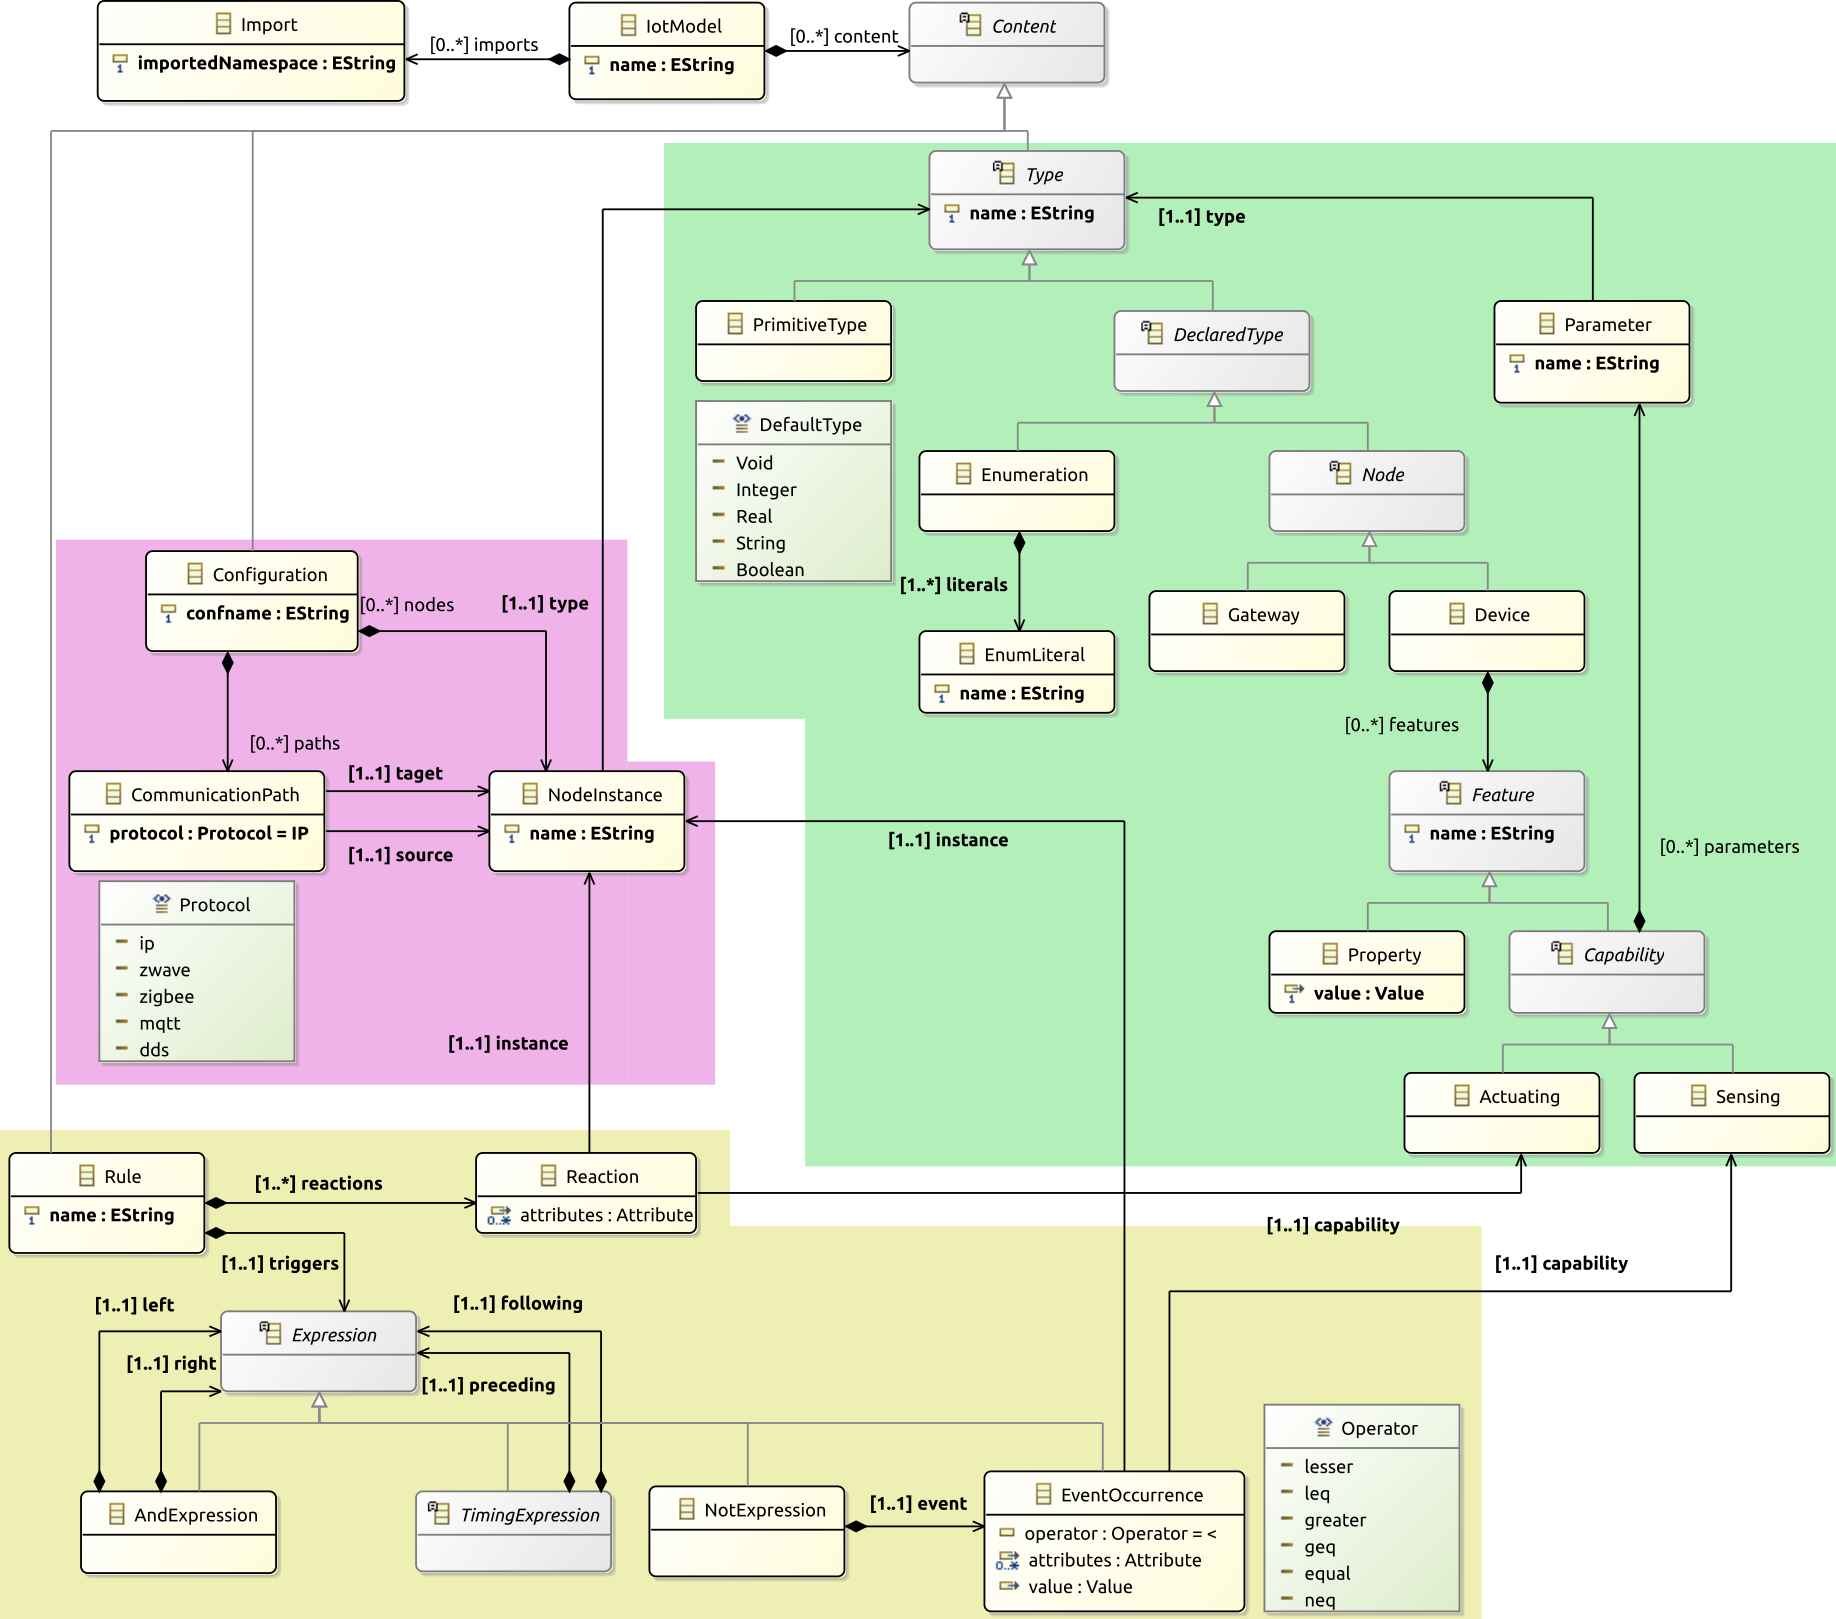
\includegraphics[width=.98\linewidth]{iotdsl-metamodel}%
  \caption{Metamodel of \IOTDSL, separated in three concerns: \emph{Type Definition} captures devices' capabilities (top-right green part), \emph{Network Configuration} details how device instances are connected to each others (middle-left purple part), \emph{Business Rules} defines the functionalities expected from the IoT installation (bottom yellow part).}%
  \label{fig:IoTDevice-MM}%
\end{figure*}

\subsection{Type Definition}
\label{sec:IoTDSL-TD}

The first task is to provide a description of which capabilities each device included in the \IOT system possess: how each device may provide information about the environment through a \emph{sensing} operation; and how it could react and influence it through \emph{actuations}. Our framework currently requires that an advanced user that is able to reason properly about how to effectively manipulate a device and extract the relevant information, but is flexible enough to accomodate automation in the future, so that information about devices could be automatically extracted from pre-existing devices databases (either from a knowledge database the \IOT system is connected to, or from a library of \emph{off-the-shelf devices}).

%In this section, we define \IOT devices' types, \textit{i.e.} which capabilities are available to the users in terms of getting information from the environment, \textit{a.k.a.} sensing, and operating on the environment, \textit{a.k.a} actuating. In our framework, type definitions either come from an advanced user who is able to reason properly about a particular device and extract the relevant information, or from a pre-existing devices database, either being a repository the system is connected to, or a library of \textit{devices-off-the-shelf}. 

\begin{figure*}%
  \centering  
  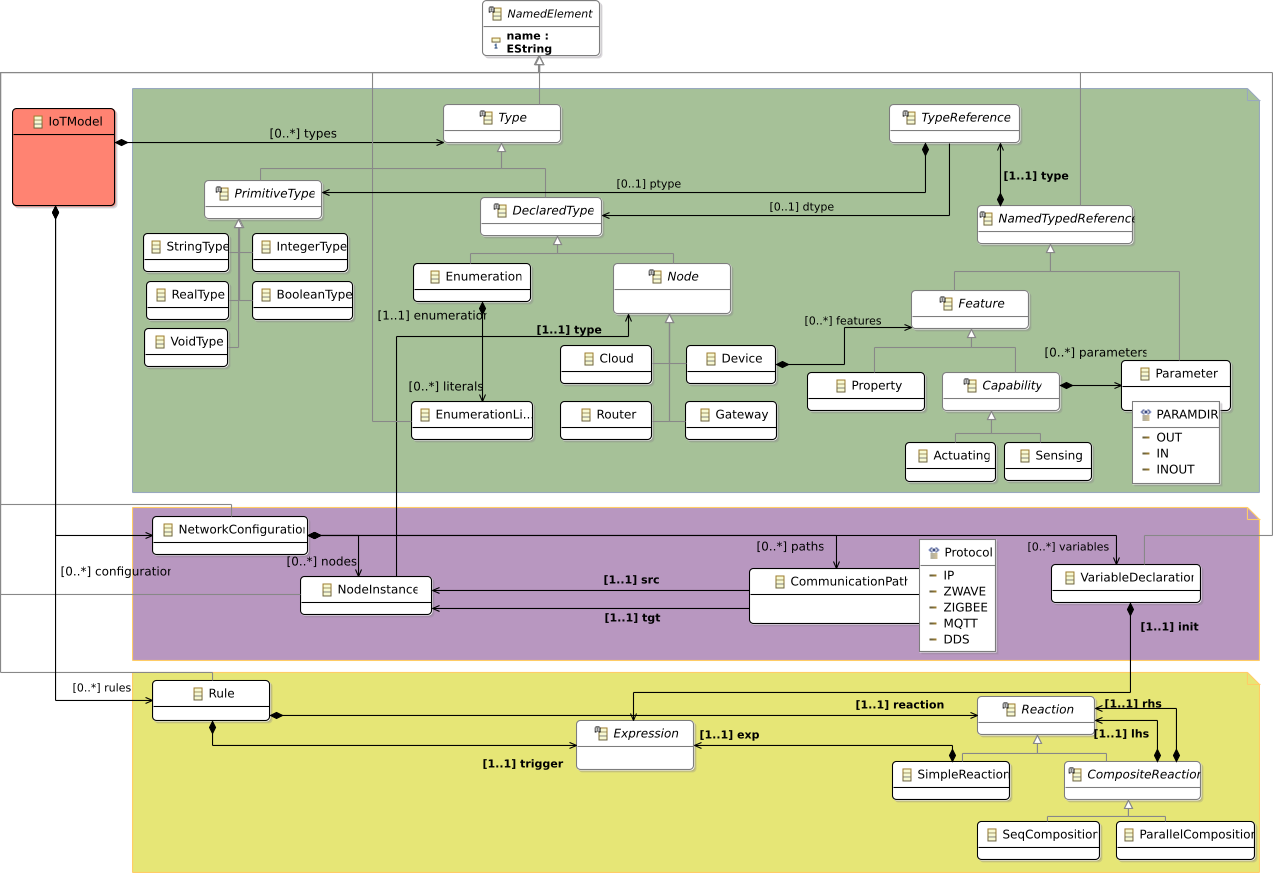
\includegraphics[width=.92\linewidth]{IoTDevice-MM.png}%
  \caption{Metamodel of \IOTDSL, separated in three concerns: \emph{Type Definition} captures devices' capabilities (top green part), \emph{Network Configuration} details how device instances are connected to each others (middle purple part), \emph{Business Rules} defines the functionalities expected from the IoT installation (bottom yellow part).}%
  \label{fig:IoTDevice-MM}%
\end{figure*}

The concepts dedicated to type definition are shown in Figure~\ref{fig:IoTDevice-MM} (green background). This part is similar to the notion of \textsf{Classifier} in \textsc{Mof}-like languages: a \textsf{Type} is either a \textsf{PrimitiveType}, or a user-defined \textsf{DeclaredType}. We distinguish between general \textsf{Gateway}s, which centralise information and processing, and \textsf{Node}s deployed in the environment and communicating with gateways, and which possess capabilities to interact with the environment. A \textsf{Capability} is basically a parameterised event that drives the node to either capture data from the environment, to act on it, or to perform both. This abstract view of an ``thing'' allows us to manipulate any device at a high abstraction level, exhibiting a clean and uniform interface for end-users based on device capabilities. Since \textsf{Node}s are \textsf{Type}s themselves, it remains possible to reference them as a parameter for the purpose of dynamic discovery across devices.

Listing~\ref{lis:RE-TypeDeclarations} illustrates how the devices in Figure~\ref{fig:scenario} are declared in \IOTDSL. Each device is introduced by the keyword \textsf{device}, possesses a name and lists capabilities that correspond to reporting events (\textsf{sensing}) or operating over the environment (\textsf{actuating}). 

\begin{table}
	\begin{minipage}[b]{.45\textwidth }%
		\begin{lstlisting}[language=iotdsl]	
gateway Middleware
device DoorDetector {
	sensing opened()
	sensing closed()
}
device MotionDetector {
	sensing moving()
}
device ToggleSwitch {
	sensing toggle()
}
		\end{lstlisting}
	\end{minipage}\hfill%
	\begin{minipage}[b]{.45\textwidth}
		\begin{lstlisting}[language=iotdsl, firstnumber=12]
		
device LightSensor {
	sensing light()
}
device LightBulb {
	actuating on()
	actuating off()
}	
device Alarm {
	actuating sound()
}
		\end{lstlisting}
	\end{minipage}
	\caption{Type declarations in \IOTDSL: capabilities as high-level events.}
	\label{lis:RE-TypeDeclarations}
\end{table}

Any IoT system should declare a special device, introduced with the keyword \textsf{gateway}, that centralises data from all devices connected to it, as we will show in Section \ref{sec:IoTDSL-NetworkConfiguration}. This device will be responsible of the event orchestration and will host the \CEP engine that embeds the implementation of the business rules. Also note that the above model is the \textit{user-defined} part of \IOTDSL. In the background, abstract events attached to all devices will need to be mapped to concrete low-level \textsc{Api}s events using a dedicated mapping language that is out of the scope of this paper.


\subsection{Network Configuration}
\label{sec:IoTDSL-NetworkConfiguration}

The configuration constructs of \IOTDSL are specified in the middle-left purple part of Figure~\ref{fig:IoTDevice-MM}. Since we use an architecture centralised around gateways, a network \textsf{Configuration} is a graph-like structure where vertices are \textsf{Gateway}s and \textsf{NodeInstance}s (so that instances may communicate with each others), while edges represent \textsf{CommunicationPath}s (or channels). Such paths define, among others, one or more protocols used to interact. We actually rely on existing platforms, such as OpenRemote (\url{http://www.openremote.org}) or SmartThings ({\url{https://www.smartthings.com}) to handle the intricate details of the protocols since such details are, from an end-user point of view, technical aspects rather than essential matters of the configuration itself. By knowing which protocols are used between each pair of devices, we can automatically perform data conversion in the proper format required by the protocols: most of those protocols are already implemented in \textit{General-Purpose Programming Languages} (\textsc{Gpl}s), like Java or C.

Listing~\ref{lis:RE-Network} shows an instantiation as well as the connection that conforms to the types given in Listing~\ref{lis:RE-TypeDeclarations} and the configuration presented in Figure~\ref{fig:scenario}.
	
	
\begin{table}
	\begin{minipage}[b]{.45\textwidth }%
		\begin{lstlisting}[language=iotdsl]	
configuration SmartHouse {
	node middle   		   : Middleware
	node alarm					 : Alarm
	node toggle          : ToggleSwitch
	node frontDoor			 : DoorDetector
	node parentDoor			 : DoorDetector
	node childDoor			 : DoorDetector
	node balconyDoor 		 : DoorDetector
	node outLight				 : LightSensor
	node livingLight		 : LightSensor
	node livingBulb			 : LightBulb
	node bathroomBulb    : LightBulb
	node foyerBulb       : LightBulb
	node balconyMotion	 : MotionDetector
	node foyerMotion  	 : MotionDetector
	node hallMotion	     : MotionDetector
		\end{lstlisting}
	\end{minipage}\hfill%
	\begin{minipage}[b]{.45\textwidth}
		\begin{lstlisting}[language=iotdsl, firstnumber=17]
	from alarm			   to middle via IP
	from frontDoor 	   to middle via IP
	from parentDoor    to middle via IP
	from childDoor     to middle via IP
	from balconyDoor   to middle via IP
	from outLight      to middle via IP
	from livingLight   to middle via IP
	from livingBulb    to middle via IP
	from bathroomBulb  to middle via IP
	from foyerBulb     to middle via IP
	from balconyMotion to middle via IP
	from foyerMotion   to middle via IP
	from hallMotion    to middle via IP
}
		\end{lstlisting}
		\vspace*{.3cm}
	\end{minipage}
	\caption{Network Configuration in \IOTDSL for our smart house.}
	\label{lis:RE-Network}
\end{table}
	
A specific device is considered as an instance of a defined type such that particular devices with the same set of capabilities may be distinguished via identifiable unique references. Communications are purely declarative and only mention the protocol type (introduced by the \texttt{\color{codeviolet}{\textbf{via}}} keyword). In our example, we simply decided to use an \textsf{IP} protocol for all bindings. Note that a similar mapping process that the one described at the end of Section~\ref{sec:IoTDSL-TD} is required to reify abstract connections between \textsf{NodeInstances} to physical ports and protocols, but again, these mapping statements are outside of the scope of this paper. 


\subsection{Business Rules}
\label{sec:IoTDSL-BusinessRules}

Business rules are the core of the manipulation of \IOT systems and compose the third part of \IOTDSL as detailed in the bottom yellow part of Figure~\ref{fig:IoTDevice-MM}. This last sub-language relies on an event-based framework that allows to specify a set of \textsf{Rule}s expressing the many functionalities an end-user wants to achieve in his/her concrete configuration. 

An \IOTDSL Business Rule is identified by the keyword \textsf{rule} followed by an unique identifier, and a body of the form << \texttt{\textbf{\color{codeviolet}{when}} trigger \textbf{\color{codeviolet}{do}} reaction} >>. Rules' \texttt{trigger}s are cyclically evaluated against the surrounding environment and specify the conditions under which the corresponding \texttt{reaction}s have to be performed to realise the end-users' scenarios. A \texttt{reaction} defines actuations on the \IOT system to send or require data of identified devices, or issues events that are internally used to synchronise rules. 

%must be triggered. Rules' \textsf{trigger}s are cyclically evaluated against the surrounding environment and a \textsf{reaction} defines a sequential or parallel combination of capabilities, enabling to sort actions by, or require data from some identifiable devices. Inside the \textsf{trigger}, users typically check events to evaluate their presences, but as we will see in the following examples, they are also able to check on their absence or returned values. A typical \textsf{reaction} may be to switch on all lights in a house, or only the ones of a certain type by sending new events.

Our approach is currently purely middleware-oriented: all rules are evaluated inside a single gateway that supposedly possesses enough processing power. We leave as future work the exploration of parallelisation techniques to support multiple gateways that communicate appropriately, or the possibility to decentralise parts of the computation into nodes with sufficient processing and power resources to optimise resource consumption and lighten communication exchanges. 

We now illustrate how the scenarios Alice is concerned about (cf. Section \ref{sec:Motivation-Scenarios}) can be translated into business rules in \IOTDSL with the devices' definitions detailed in Listings~\ref{lis:RE-TypeDeclarations} and \ref{lis:RE-Network}. 

\begin{description}[leftmargin=0cm]
	\item[Switching entrance lights on when coming in]  When Alice gets home (and thus opens the front door), she wants the lights to be automatically switched on in the foyer and in the living room.
	\begin{lstlisting}[language=iotdsl,
							label=lis:home-rule,
		caption=Rule to switch on the lights at home incoming]
rule SwitchLightsWhenEntering:
	when (foyerMotion.moving after frontDoor.opened) do {
		foyerBulb.on
		livingBulb.on
	}
	\end{lstlisting}
	This rule introduces what we call \emph{facilitators}, i.e. keywords that define an unspecified time window in which a sequence of events should be observed. This time window is system-specific and needs to be defined independently in configuration files independent of descriptions in \IOTDSL. In this case, the \inlineI{foyerMotion} should detect movement \emph{nearly after} the \inlineI{frontDoor} detects an opening. 
		
	Note that reactions are defined as a sequence that does not matter: the order in which the \inlineI{foyerBulb} and the \inlineI{livingBulb} switch on largely depends on the platform capacities, i.e. they can be actuated synchronously or sequentially (in which case, no guarantee is given that the definition order will be respected). At the abstraction level \IOTDSL operates, it is irrelevant since the end user wishes to see both switched on at some point, without having to consider low-level details that would enforce such behaviour.

	\item[Illuminate bathroom when children wake up at night] When Alice's little boy wakes up at night, she would like to have the light in the bathroom to be switched on to prevent him from falling or injuring himself. Analogously, she wants the light to be switched off when he gets back to sleep afterwards.
	\begin{lstlisting}[language=iotdsl,
							label=lis:night-rule,
		caption=Rules to switch on\//off lights in the corridor at night]
rule SwitchBathroomLightOnAtNight:	
	when (not livingLight.light and 
	 (hallMotion.moving after childDoor.opened)) do {
		bathroomBulb.on
	}

rule SwitchBathroomLightOffAtNight:	
	when (not hallMotion.moving within 3 min from childDoor.closed) do {
		bathroomBulb.off
	}
	\end{lstlisting}
	The rule \inlineI{SwitchBathroomLightOnAtNight} introduces a new keyword \inlineI{not}, which represents the \emph{absence} of a certain event type, here \inlineI{livingLight.light}. This is different than simply observing some events occuring. Note also that the second part of the rule trigger uses parenthesis to relate the facilitator \inlineI{after} to the closest event \inlineI{childDoor.open}, instead of spanning on the whole condition.

	The rule \inlineI{SwitchBathroomLightOffAtNight} presents a combination of negation with an explicit time window with the construct \inlineI{within ... from}: it indicates that no event of type \inlineI{movement} from the hall motion sensor should occur in a three-minute time window after observing the \inlineI{closed} event from the boy's door, in order to trigger the rule. \IOTDSL defines several useful time units to cope with simpler definitions (seconds, minutes, hours, or a combination of the three). 
	

	\item[Report unsupervised children on balcony] Alice considers that it is a critical situation if a child enters into the balcony without her knowledge, because of fall risks. To avoid that, she placed a switch button high enough that only an adult could press when accompanying a child outside. If the button is not pressed within 3 seconds after someone enters the balcony, an alarm should sound.
	\begin{lstlisting}[language=iotdsl,
							label=lis:balcony-rule,
		caption=Rules to sound the alarm in case of an unsupervised child on the balcony]
rule AlarmWhenChildOnBalcony:	
	when (not toggle.toggled within 5 sec from 
			(balconyMotion.moving after balconyDoor.opened)) do {
		alarm.sound
	}
	\end{lstlisting}
	This last rules states that once the balcony door has been opened and movements are detected on the balcony, the alarm should sound unless the toogle button is pressed in a five-second time window. This rule is similar to \inlineI{SwitchBathroomLightOffAtNight}, except that the baseline of the time window is here a composite event using a facilitator: once an opening followed by movements on the balcony is observed, we expect the toggle button to be pressed. 
\end{description}

To summarise, an end-user uses the Business Rules sublanguage to specify the scenarios of interest in the form of \inlineI!when (trigger) do {actuations}!: the \inlineI{trigger} condition specifies the event (non-) occurrence pattern under which the \inlineI{actuations} are performed, by using common boolean connectors as well as time windows to observe delayed events; whereas the \inlineI{actuations} are undeterministically performed independently to their definition order. 

From a qualitative point of view, adopting a rule-based language presents the advantage of mimicking the cognitive process of establishing a scenario, which should ease the adoption of \IOTDSL. However, we are conscious that this requires a further examination and actual validation with end-users that are not aware of the underlying \DSL mechanisms, but we believe that presenting a visual representation for rules and powerful analysis of rule activation could ease the adoption process and facilitate scenario definitions.







\section{Related Work}
\label{sec:RW}

A series of overviews have been recently conducted on several aspects of \IOT. In \cite{alfuqaha-15,xu-14a}, the authors reviewed the applications, protocols and technologies used in the distinct \IOT layers, while \cite{singh-14,gubbi-13} focused on architectural aspects and \cite{tan-10,xu-14b} reviewed security ones. Most of these contributions identify a number of challenges crossing the application domain of a \DSL for \IOT, from which we identified the most relevant ones to our contribution in Section~\ref{sec:Motivation} and to which we confront our framework in Section~\ref{sec:Discussion}.

Capturing variations of a domain with explicit constructs close to the domain concepts resides at the essence of \DSLS. In that regard, many \DSLS were proposed for various purposes in the \IOT stack. \textsc{Chariot}~\cite{pradhan-15} addresses Cyber-Physical Systems by providing a component model that clearly distinguishes between communication and computation, while ensuring resilience features in highly reconfigurable systems. In~\cite{brandtzaeg-12} is presented a \DSL aimed at facilitating the deployment of applications, based on a component model of the environment used to locate the architecture nodes where business logic can be leveraged. \textsc{Alph}~\cite{munnelly-08} is a \DSL for ubiquitous healthcare that focuses on three concerns: mobility, by helping users to manage frequent devices disconnections; context-awareness to adapt application behaviour to environmental changes; and infrastructure, for managing the heterogeneity of communication protocols. Midgar~\cite{garcia-14} offers a visual interface to support end-users in controlling interconnected devices and generate the glue application making these devices interoperate. In~\cite{salihbegovic-15}, the authors present a visual \DSL for capturing the features and intercommunications of devices distributed in various application domains spanning from smart homes to patient monitoring. These contributions target different application domains at different abstraction levels, but possess every key features we identified in Section~\ref{sec:Motivation} in a more or less explicit way. Since \IOTDSL targets end-users with no prior knowledge in programming, we contrast with these contributions by offering a more intuitive, declarative style for expressing the system's dynamics through semantics rules that are compilable into a runnable \CEP engine.

ThingML~\cite{harrand-16} is the closest contribution to our \DSL: it uses a similar device description with messages and communication ports attached to devices, but describes the dynamics of devices and systems through state machines, which appear to be more obscure for end-users. However, the conceptual drawbacks are similar in both paradigms: state machines need to be deterministic on their transitions, while rules have to avoid multiple concurrent firing to avoid executing several rules at the same time. 

Other approaches, \textit{e.g.}~\cite{bhandari-13,cheng-16}, relying on the \textit{Event Condition Action} (ECA) paradigm, share a similar view for \IOT devices orchestration through \CEP, though not having the same expressiveness for devices' definition as we propose, especially with time frames and event compositions. In~\cite{shimokura-07}, the authors add \textit{pre-} and \textit{post-conditions} to ECA rules but they still do not address time frames constraints.

All previous contributions take advantages of \MDE technologies and tools. More general \MDE framework like GeMoC~\cite{bousse-16} or ThingML allow to specialise the description of interconnected devices, for example to describe Arduino systems specifically in ArduinoML~\cite{mosser-14}. On contrary, \IOTDSL framework concentrates on generating executable rules from user-defined requirements.
\section{Conclusion and Future Work}
\label{sec:Conclusion}

In this paper, based on recent research, we summarised the needed features as well as major challenges for the adoption of a specific language for \IOT systems. We introduced \IOTDSL, a domain specific language, designed to tackle those various challenges, \textit{e.g.} in terms of capability discovery, event processing or interoperability. In \IOTDSL, devices are described in a common \textit{Classifier} - \textit{Type} - \textit{Instance} layered specification that allows modellers to easily distinguish between typing and running instances concepts. A second benefit of that separation is the ability to create reusable \textit{libraries} of conceptual components, so \IOT devices by extension. By raising the abstraction level and hiding technical constraints to end-users, \IOTDSL is designed to serve as a handy modelling mean for them. Moreover, by abstracting the communication complexity into dedicated modelling construct, it is aimed to facilitate future evolution and re-configuration of existing solutions, since device descriptions may be retrieved from a centralized gateway.

Behavioural specifications are key aspects in \IOTDSL. We decided to rely on event-based \textit{rules} instead of state machines for their conciseness and readability, though rules may be converted to state machines automatically. Together with high-level \textit{operations} descriptions, they offer a more concise mean to describe dynamic aspects of \IOT configurations, without loosing formal model verification capabilities.

However, the prototype language is at early development stage and some features are currently missing or under development. First, the expression language must be validated on a real world examples and the mapping layer in charge of reconciling the abstract definitions and the technological APIs. Second, the complex composition of rules must be further investigated. Last, we plan to investigate on logic migration possibilities from the gateways to nodes with sufficient capacity. 
%\vfill
\bibliographystyle{apalike}

{\small \bibliography{./MODELSWARD2017.bib}}


\end{document}